\chapter{Search for the $\hmumu$ decay}

\textit{"The Higgs boson may, or may not, couple to the second generation fermions."}

\vspace{5mm}
\begin{flushright}
--- a bright bunch of ATLAS scientists.
\end{flushright}

\thispagestyle{empty}
\newpage

The interactions between the Higgs boson and the vector bosons and
third generation fermions, critical to the discovery in 2012, soon 
became the preferred way to study the properties of the Higgs boson.
The mass \cite{Aad:2015zhl, Aaboud:2018wps, CMS-PAS-HIG-19-004},
as well as inclusive and differential cross-sections
\cite{Aad_2015, Chatrchyan_2014, Aaboud:2017oem, Sirunyan:2018sgc, Aaboud:2018ezd},
have been measured and new production modes, $\tth$ \cite{Sirunyan:2018hoz, Aaboud:2018urx}
and $\vh$ \cite{Sirunyan:2018kst, Aaboud:2018zhk}, have been 
observed. However, the interactions between the Higgs boson
and the first or second generation of fermions have not been
observed yet due to experimental challenges. In the leptonic
sector the main challenge is a very small branching fraction due
to the small mass of electron and the muon compared to the tau.
In the quark sector some branching ratios, for example to the charm
quark pair, are larger than those in which the Higgs was discovered.
However, detection is experimentally difficult in the LHC environment
due to the difficulty in flavour tagging, and estimating and modelling
backgrounds \cite{Aaboud:2018fhh, CMS-PAS-HIG-18-031}. Ultimately the
decay to muon pairs offers the best sensitivity to probe the
interactions between the Higgs boson and the second generation
fermions.

In the Standard Model the branching ratio of the Higgs boson with a
mass of 125.09 \GeV~is predicted to be $2.17 \times 10^{-4}$
\cite{deFlorian:2016spz}. This could be modified by physics beyond the
SM \cite{Giudice:2008uua, Dery:2013rta, PhysRevD.80.095023}, meaning
that any deviation from the predicted value could be a sign of new
physics.

ATLAS and CMS experiments have already conducted searches using
the LHC Run 1 data collected at centre-of-mass energies $\sqrts = 7$
and 8 \TeV, both setting the 95\% confidence level upper limits on the
product of the Higgs production cross-section and the branching ratio
to muon pairs \cite{Aad:2014xva, Khachatryan:2014aep} of about seven
times the SM expectation. Using the data collected at $\sqrts = 13$
\TeV, in years 2015 and 2016 the observed upper limit was further
decreased to 2.8 and 2.9 by ATLAS and CMS respectively
\cite{Aaboud:2017ojs, CMS-PAS-HIG-17-019}, with ATLAS
further updating its result to 2.1 using the data collected in 2017
\cite{ATLAS-CONF-2018-026}. This corresponds to $0.9 \sigma$ expected
significance, meaning that the channel is on the verge of evidence.

This chapter presents the search for the Higgs boson decay to muon
pairs using full ATLAS Run 2 dataset collected between 2015 and 2018
at $\sqrts = 13$ \TeV, almost doubling the integrated luminosity of
the dataset since the last result to $139~\ifb$. The Higgs boson mass
is assumed to be 125.09 \GeV~for all presented results.

The overall strategy of the analysis is to select events with
two oppositely charged muons passing the single muon triggers,
and apply additional requirements
to reduce $\ttbar$ and diboson backgrounds. Events are then split
in three channels based on whether they contain zero, one, or two or
more jets in addition to the muon pair. They are further split in
individual categories using a multivariate discriminant, based
on the differences in kinematics between the muon pairs coming
from a Higgs boson produced in the main production modes, and the
muon pairs coming from background events, which are dominated by
the Drell-Yan spectrum. Signal events tend to be more central and
have higher transverse momentum, their jet multiplicity is higher,
and the VBF production mode has a unique signature of two 
back-to-back high-$\pt$ jets with little hadronic activity between
them. Finally, a maximum likelihood fit to the dimuon invariant mass
spectrum is performed in all categories simultaneously, extracting
the signal strength parameter. The analysis is limited by
statistical uncertainty arising from a limited size of the dataset.
The systematic uncertainties are dominated by the uncertainty on
the background modelling, assessed using a dedicated simulated sample.
Additional systematic uncertainties arise from the normalisation 
of signal sample and migration between the categories, such as
the uncertainty on the production cross-section and branching ratio
from the theoretical side, and luminosity, muon momentum resolution
and detector calibration from the experimental side.

A number of improvements were introduced with respect to the
previous result. Selection was improved by including additional
muons from the corners of detector acceptance, by improving
the resolution of the invariant mass by recovering the final
state radiation, and by better rejection of \pileup~ jets in the
forward region. The allocation of events in the categories was
improved by employing a fully multivariate approach in lieu
of a hybrid approach combining a multivariate discriminant and 
cut-based categories. Finally, the background modelling was
improved by using a new functional form and larger DY simulation
dataset. The total effect of all improvements is an approximately
20--30\% increase in the analysis sensitivity and is dominated
by the improvements from using a fully multivariate categorisation
approach.

\section{Data and MC simulation samples}

The proton-proton collision data used in this analysis was
collected in 2015, 2016, 2017, and 2018 at the centre-of-mass
energy of 13 \TeV~in the main physics stream. It corresponds
to an integrated luminosity of 139 $\ifb$ after passing the data
quality checks which ensure that the important parts of the
detector are switched on and function as intended.

The MC simulation samples are used in the analysis for a 
variety of purposes. The signal samples are used to optimise
the event selection and to determine the normalisation and
shape of the signal model in the analysis categories.
Centrally produced background MC simulation samples are used
to optimise the event selection and to validate the muon
momentum resolution in the analysis categories, but not to
determine the normalisation or shape of the backgrounds.
While the normalisation and shape parameters are determined
in the final fit to data, the functional form is selected
in each analysis category independently using a custom
high-statistics MC simulation of Drell-Yan events.

\subsection{Background samples}

\label{sec:bkg-mc}

The leading irreducible background for the analysis is the
Drell-Yan (DY) production of muon pairs. It is simulated using
\textsc{Sherpa} 2.2.1 with the NNPDF3.0 set of parton
distribution functions (PDF) \cite{Ball:2014uwa} in slices of
$\HT$ and with $c$- and $b$-quark filters, simulating 0--2
jet events at next-to-leading order (NLO) and at leading order
(LO) for 3 and 4 jets using \textsc{Comix} \cite{Gleisberg:2008fv}
and \textsc{OpenLoops} \cite{Cascioli:2011va, Denner:2016kdg}
libraries. Matching with the \textsc{Sherpa} parton showering
\cite{Schumann:2007mg} is done using the MEPS@NLO prescription
\cite{Catani:2001cc, Hoeche:2012yf, Hoeche:2011fd}.
In order to populate the tails of the
DY invariant mass distribution relevant for the analysis an
additional high-statistics sample is generated with identical
setup an an additional cut of $\mmumu > 100$ \GeV. Finally, 
\textsc{Sherpa} is also used to model the electroweak $Z$+jets
process with up to two additional jets at LO accuracy beyond
the first two jets.

With the mass of the top-quark set to $m_t = 172.5$ \GeV, the
$\ttbar$ and single-top samples are generated using
\textsc{Powheg-Box} \cite{powheg, Frixione_2007, Alioli_2010}
with NNPDF3.0 PDF set and parton showering and hadronisation
done in \textsc{Pythia} 8.186 using the A14 parameter set
\cite{ATL-PHYS-PUB-2014-021}. $\ttbar$ cross-section is
computed to next-to-next-to-leading order (NNLO) in
QCD with next-to-next-to-leading logarithmic
(NNLL) soft gluon terms taken into account. The cross-section
of the single-top is computed with prescriptions from
\cite{Kidonakis:2011wy, Kidonakis:2010ux}, and all the processes
($t$-channel, $s$-channel, and $Wt$-channel) are generated
separately.

Diboson processes, $WZ$ and $ZZ$, are generated using
\textsc{Sherpa} 2.2.1 with the NNPDF3.0 PDF set, and are normalised
directly to the \textsc{Sherpa} prediction. Only semi-leptonic
and fully-leptonic decays are simulated.

\subsection{Signal samples}

The largest contribution comes from the $\ggf$ signal sample,
generated with \textsc{Powheg-Box} with PDF4LHC15 PDF set
to next-to-next-to-leading order accuracy with parton shower matching
(NNLOPS) \cite{Hamilton:2013fea}, achieving NNLO in QCD after
the re-weighting in rapidity of the Higgs boson. The cross-section
for the $\ggf$ production mode are computed to
next-to-next-to-next-to-leading order (N3LO) \cite{Anastasiou:2016cez}
in QCD with NLO electroweak corrections applied
\cite{Aglietti:2004nj, Actis:2008ug} under the assumption that
they factorise. \textsc{Pythia} 8 with the AZNLO parameters
\cite{Aad:2014xaa} is used to simulate the decay
of the Higgs boson, final state photon radiation, parton
showering, and hadronisation. 

$\vbf$ and $q\bar{q}/qg \rightarrow \vh$ production modes are
generated to NLO accuracy in QCD using \textsc{Powheg-Box},
while the $gg \rightarrow ZH$ is generated to LO accuracy. Same
PDF set and \textsc{Pythia} tunes are used as in the $\ggf$
generation. VBF cross-section is computed with full NLO QCD
and electroweak corrections \cite{Ciccolini:2007jr, Ciccolini:2007ec,
Arnold:2008rz}, and approximate but highly accurate NNLO QCD
corrections \cite{Bolzoni:2010xr}. VH cross-section is computed at
NNLO in QCD \cite{Brein:2003wg} with NLO eletroweak
corrections \cite{Ciccolini:2003jy}, apart from the
$gg \rightarrow ZH$ which is computed to NLO and next-to-leading-logarithm
accuracy in QCD \cite{Ciccolini:2003jy, Brein:2003wg, Brein:2011vx,
Altenkamp:2012sx, Denner:2014cla, Brein:2012ne, Harlander:2014wda,
Harlander:2018yio}.

$\tth$ production mode is generated using \textsc{MadGraph5\_aMC@NLO}
\cite{Alwall:2014hca, Artoisenet:2012st} at NLO accuracy using
NNPDF3.0NLO PDF set and the A14 tune. The cross-section is
computed to NLO in QCD with NLO electroweak corrections
\cite{Yu:2014cka, Beenakker:2002nc}.

\textsc{Pythia} is also used to
overlay minimum bias events to model the effects of \pileup~for all
simulated events using the NNPDF2.3LO PDF set \cite{Ball:2012cx}
with the A3 parameters \cite{ATL-PHYS-PUB-2016-017}. All signal
and background samples are passed through the full ATLAS
detector simulation. Pile-up re-weighting, object momentum
smearing, and efficiency scale factors are applied to the MC
simulation samples in order to make them mimic the collected data.

\subsection{Custom Drell-Yan sample}

Extract the signal strength paramater relies on a
maximum likelihood fit to the invariant mass spectrum in data,
using parametrised models of both signal and background. The choice
of the functional form describing the background is crucial because
a mismodelling of the background results in a bias on the extracted
signal strength. This is particularly significant when the
signal-to-background ratio is very small, because the impact can be
large.

In order to select the functional form and evaluate the resulting
bias, referred to as the ``spurious signal", a fit to the
background-only spectrum is performed. Ideally, this would be done
on the background MC simulation described in Section \ref{sec:bkg-mc},
but because of the high computational cost associated with the 
simulation of the detector response the statistics of the sample
are on the same order of magnitude as the data. As a result, the
the extracted spurious signal value is unreliable and dominated by
the statistical fluctuations. A custom high-statistics sample of DY
events is generated to overcome this challenge.

The custom DY sample needs to have significantly larger statistics
than the data, requiring a much faster generation. To facilitate
this, the sample is produced at a generator-level only, skipping
the simulation of showering, hadronisation, and detector response,
replacing them by parametrised smearing functions. The effect on
the dimuon invariant mass spectrum is minimal, and because of the
parametrised smearing the jet mismodelling is a second order effect.
On the other hand, final state radiation (FSR) does have an effect on
the invariant mass spectrum and is simulated by \textsc{Photos++}
\cite{Golonka:2006tw}. This setup was fast enough to generate 20
billion events corresponding to approximately 100 $\iab$ in the 
regions of parameter space relevant for the analysis. A drawback of
the sample is that it only models the dominant DY part of the
invariant mass spectrum.

At generator level, the samples are produced separately for zero
or one parton and two partons in addition to the muon pair:
\begin{itemize}
\item \textsc{Powheg} is used to generate an inclusive NLO $\zmumu$
sample, modelling zero and one parton in addition to the muon pair.
For efficiency reasons two sub-samples are generated, one with
$60 < \mmumu < 95$ \GeV~($2.5\times10^{9}$ events), and the other
with $\mmumu > 95$ \GeV~($10\times10^{9}$ events) requirement. Even
after detector smearing the latter sample dominates the fit region.
\item \textsc{Alpgen} \cite{Mangano:2002ea} is used to generate
events with two partons in addition to the muon pair at LO. The 
computation uses only the matrix element with two additional
partons and requires both of them to have $\pt > 25$ \GeV~as well
as $\Delta R(j,j) > 0.4$ to minimise the overlap with the
\textsc{Powheg} sample. Similarly to the \textsc{Powheg} sample,
events are generated with $60 < \mmumu < 95$ \GeV~($1.75\times10^{9}$
events) and $\mmumu > 95$ \GeV~($2.5\times10^{9}$ events)
requirements. These events are crucial to populate the analysis
categories with a large fraction of the signal events coming from
the VBF production mode.
\end{itemize}
Both samples are corrected in the same way to model the effects of
the detector. Muon momentum smearing is done using parametrised functions
derived from MC simulation described in Section \ref{sec:bkg-mc}.
Effects from identification, reconstruction, isolation, and impact
parameter efficiencies are also derived from MC simulation and 
applied as weights, while trigger efficiency weights are derived
from data. FSR momentum is smeared using parametrised prescription
from the ATLAS subgroup specialising in electrons and photons.
Photons are dropped randomly to emulate the reconstruction
efficiency. Smearing of jet momenta is performed using the parametrisation
from the ATLAS subgroup specialising in jets and missing energy.
The effect of \pileup~jets is modelled by building a library of
jets from minimum-bias events in MC simulation and overlaying a
number of sampled jets from the library for each event. A dedicated
missing transverse momentum smearing is derived from the Run 2 data.

\section{Physics objects}

The search for a narrow resonance on top of a smoothly falling
background appears at first sight to require not much more than an
excellent understanding of muons in ATLAS. While the intirety of Chapter
\ref{sec:muons} is dedicated to their performance, the sophistication
of the analysis requires understanding of other objects as well.
Photons are used to recover the final state radiation in order to improve
the resolution of the invariant mass spectrum. Jets are used
as a handle to select events produced in the VBF production mode
and to improve separation from the other backgrounds. Even electrons
are reconstructed, albeit solely in order to reject fake jets. Finally,
missing transverse momentum ($\met$), is used to supress top and diboson
backgrounds.

\subsection{Muons}

Muon reconstruction, identification, and isolation are described in
detail in Chapter \ref{sec:muons}. Table \ref{tab:hmumu:muons}
summarises the selection used for the $\hmumu$ analysis.
\begin{table}[h]
\centering
\caption{Summary of the muon selection requirements.}
\label{tab:hmumu:muons}
\begin{tabular}{c c}
\toprule
\midrule
ID selection & Loose \\
\midrule
Isolation selection & FixedCutPflowLoose \\ 
\midrule
$\pt$  & $\pt > 15$ \GeV \\
\midrule
$\eta$ & $|\eta| < 2.7$ \\
\midrule
\multirow{2}{*}{Impact parameters} & $|d_0 / \sigma_{d_0}| < 3.0$ \\
                                   & $|z_0 \cdot \sin{\theta}| < 0.5$ mm\\
\midrule
\bottomrule
\end{tabular}
\end{table}
The majority of reconstructed muons in the Loose selection are
the CB type, combining the information from the tracker and
muon spectrometer systems. However, in order to maximise the
acceptance of signal events other muons types are also used
to improve the reconstruction efficiency in the challenging
parts of the detector. ST and CT improve the reconstruction
efficiency in the $|\eta| < 0.1$ region where the muon
spectrometer has a gap to allow for cabling and services to
the tracker, while the ME muons are used in the forward
regions to reconstruct muons outside of the tracker
coverage, where $2.5 < |\eta| < 2.7$.

CB muons benefit from a combination of two $\pt$ measurements,
the one in the tracker, and the one in the muon spectrometer.
Figure \ref{fig:hmumu:reso} verifies that the resulting dimuon
invariant mass resolution is only marginally worse for muon
pairs containing one non-CB muon (dotted green line) compared
to pairs where both muons are CB (dashed blue line). Since
most muons are CB, the inclusive distribution (solid orange
line) and the distribution of purely CB muons (dashed blue line)
are nearly identical.

The reason for such a small degradation is that the resolution of the combined
$\pt$ measurement is dominated by the tracker $\pt$ measurement
in the barrel region, and by the muon spectrometer measurement
in the forward regions. ST and CT muons, used in the $|\eta| <
0.1$ region, combine a track in the ID with a segment in the
muon spectrometer or with a calorimeter deposit, and thus 
benefit from having the high-quality tracker $\pt$ measurement.
Conversely, ME muons, used in the $2.5 < |\eta| < 2.7$ region,
use the track from the muon spectrometer, the higher quality
measurement in the forward region.
\begin{figure}[h!]
  \centering
  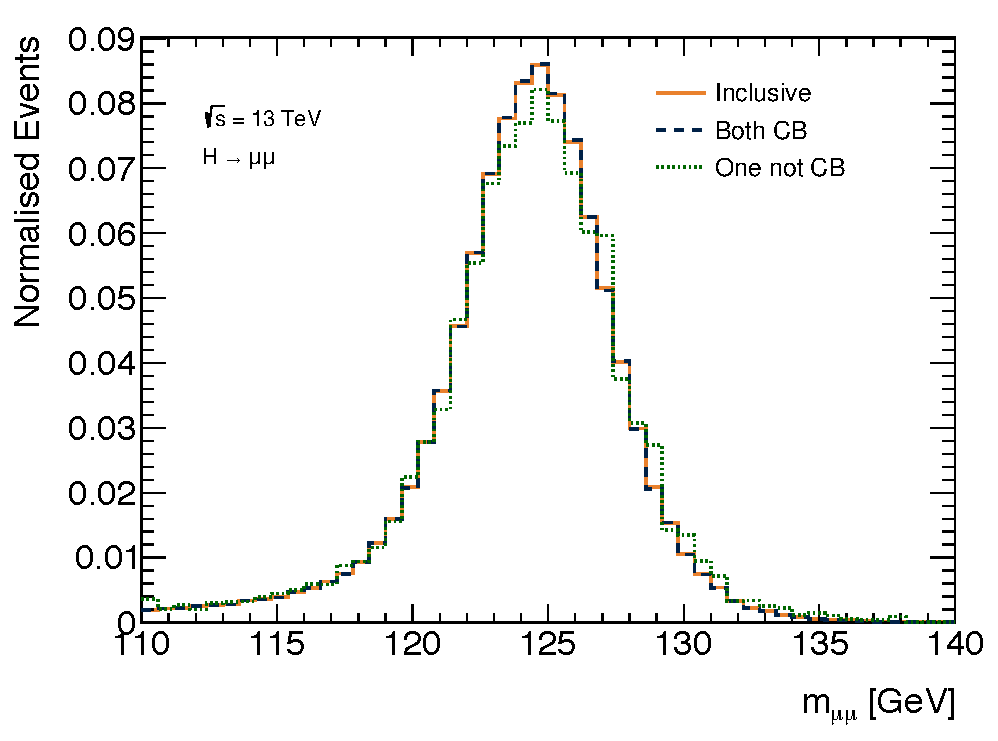
\includegraphics[width=0.8\textwidth]{figures/hmumu/resolution}
  \caption[Muon resolution for different muon types]{Resolution
  of the dimuon invariant mass measurement for the $\ggf$ signal
  sample in the $\hmumu$ analysis signal region. Events in which
  both muons are CB type are shown in dashed blue line, while
  events in which one of the muons is not CB are shown in dotted
  green line. Inclusive distribution is shown in the solid orange
  line.}
  \label{fig:hmumu:reso}
\end{figure}
The FixedCutPflowLoose isolation selection is used because
of a combination of its high efficiency, robustness to high
\pileup~conditions, and an improved rejection of heavy-flavour
jets. The cut on the $\pt$ rejects muons from the decay of
heavy-flavour quarks, while cosmic rays are rejected by the
standard requirements on the impact parameters.

\subsection{Photons and FSR}

Photons are reconstructed in ATLAS via its energy deposits
in the eletromagnetic calorimeter. Unlike electrons, photons
are electrically neutral and do not leave tracks in the
tracker, unless they are converted to electron-positron
pairs before reaching the calorimeter. The details on the
reconstruction algorithm and its performance are described
in Ref. \cite{Aaboud:2018yqu}.

Muons may radiate a photon and thus lose energy, meaning that
the invariant mass of the muon pair is no longer equal to the
mass of the mediator. In order to mitigate this effect up to
one final-state photon candidate is added to the mass
calculation, using a procedure similar to the one used in
Ref. \cite{Aad:2014eva}, but optimised for the high-purity
requirements of this analysis. Collinear photons
($\Delta R(\gamma, \mu) < 0.20$) are required to have $\pt$
larger than a linearly increasing threshold, from
$\pt^\gamma > 3$ \GeV~at $\Delta R(\gamma, \mu) = 0$ to
$\pt^\gamma > 8$ \GeV~at $\Delta R(\gamma, \mu) = 0.2$.
Non-collinear photons ($\Delta R(\gamma, \mu) > 0.20$)
are required to have $\pt^\gamma > 8$ \GeV~and tight \cite{Aaboud:2018yqu}
identification requirement for photons. When multiple
photon candidates are found only the one with the highest $\pt$
is included in the invariant mass calculation, with priority
to the collinear photons over non-collinear ones.

Around 5\% of all signal events have at least one FSR candidate,
of which approximately 90\% are the collinear photons.
The distribution of invariant mass for the MC simulation of
$\ggf$ signal events with at least one reconstructed FSR
candidate is shown in Figure \ref{fig:hmumu:fsr}
before and after the recovery of final state radiation.
It can be seen that the mass peak is shifted much closer to
125 \GeV, with the slight overshoot resulting from the fake
FSR candidates coming from pileup. The improvement in the
invariant mass resolution is approximately 3\% inclusively.
A drawback of the FSR recovery is an $\sim 8\%$ increase in the
number of background events in the signal region due to the
migration of events from the $Z$ mass peak.
\begin{figure}[h!]
  \centering
  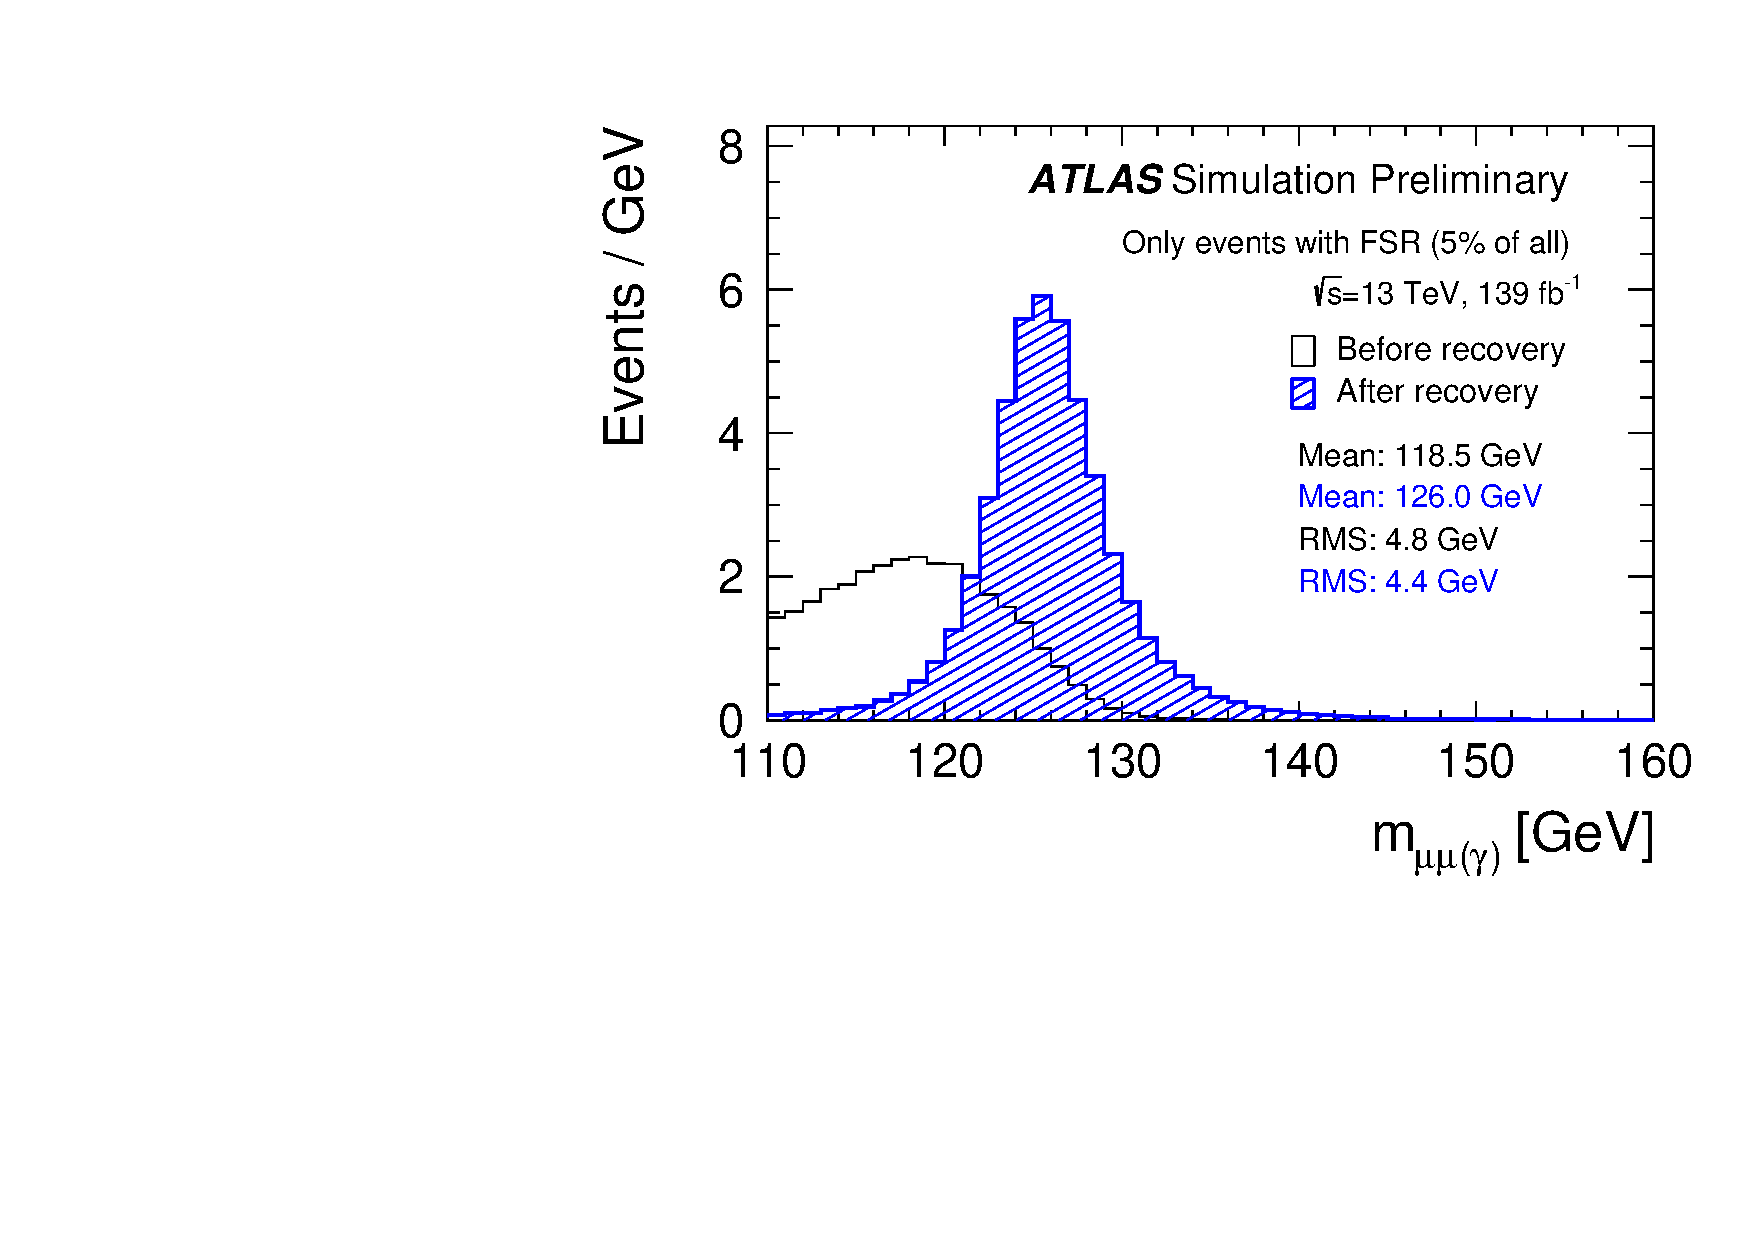
\includegraphics[width=0.8\textwidth]{figures/hmumu/FSR_fsr}
  \caption[Final state radiation recovery]{Invariant mass before
  (white solid) and after (blue hatches) final-state radiation
  recovery for a MC simulation of $\ggf$ signal events passing
  the analysis selection. Only events with one or more
  reconstructed FSR candidates are shown. The mean and the
  root-mean-square of the distributions are shown in the bottom
  right corner. From Ref. \cite{ATLAS-CONF-2019-028}.}
  \label{fig:hmumu:fsr}
\end{figure}

\subsection{Jets, electrons, and $\met$}

Jets are the collimated collections of hadrons, arising either
from a parton in the final state of the interaction, the remnants
of the proton not participating in the hard scatter (underlying event),
or from \pileup~interactions. They are used to identify events
which could have been produced via the VBF production mode by
exploiting its typical dijet signature. Jets are experimentally the richest
objects in ATLAS, reconstructed either from the deposits in the
calorimeters, tracks that the charged hadrons leave in the tracker,
or both. The optimal use of substructure has been extensively
studied both theoretically \cite{Altheimer:2012mn} and using
a wide variety of modern machine learning techniques \cite{Larkoski:2017jix}.
The reconstruction used in this analysis is based on topological
clusters of calorimeter cells \cite{Aad:2016upy}, which are used as
an input to the anti-k$_\text{T}$ clustering algorithm
\cite{Cacciari:2008gp, Cacciari:2011ma} with the distance parameter
$\Delta R = 0.4$. A requirement on the jet $\pt > 25$ \GeV~for the
central jets ($|\eta| < 2.5$), and at $\pt > 25$ \GeV~for the forward
jets ($2.5 < |\eta| < 4.5$).

The suppresion of jets coming from \pileup~ is achieved by using a
dedicated jet vertex tagging (JVT) discrimant \cite{ATLAS-CONF-2014-018},
constructed using tracking information. In the forward region \pileup~
jet suppression is achieved with the fJVT discriminant \cite{Aaboud:2017pou},
using the information on jet shape and the topological correlations in
\pileup interactions.

Jets containing a $b$-hadron are identified using a multivariate
$b$-tagging algorithm \cite{Aaboud:2018xwy} if they are inside the
tracker ($|\eta| < 2.5$). A selection providing 60\% tagging
efficiency for real $b$-jets and less than 0.1\% fake rate for
light-flavoured jets \cite{ATL-PHYS-PUB-2017-013} is used
to tag the jets.
\begin{table}[h]
\centering
\caption{Summary of the jet selection requirements.}
\label{tab:hmumu:jets}
\begin{tabular}{c c}
\toprule
\midrule
Algorithm              & Anti-k$_\text{T}$ ($\Delta R = 0.4$)\\
\midrule
$\eta$                 & $|\eta| < 4.5$ \\
\midrule
\multirow{2}{*}{$\pt$} & $\pt > 25$ \GeV~for $|\eta| < 2.4$ \\
                       & $\pt > 30$ \GeV~for $2.4 < |\eta| < 4.5$ \\
\midrule
\multirow{2}{*}{JVT}   & JVT $> 0.59$ \GeV~for $|\eta| < 2.4$ and $20 < \pt < 120$ \GeV \\
                       & JVT $> 0.11$ \GeV~for $2.4 < |\eta| < 2.5$ and $20 < \pt < 120$ \GeV \\
\midrule
fJVT                   & fJVT $< 0.5$ \GeV~for $2.5 < |\eta| < 4.5$ and $20 < \pt < 120$ \GeV \\
\midrule
b-tag                  & MV2c10 60 WP for $|\eta| < 2.5$ and $\pt>20$ \GeV \\
\midrule
\bottomrule
\end{tabular}
\end{table}
Electrons are reconstructed by matching a track in the ID with a
calorimeter deposit in the ECAL, as described in Ref. \cite{Aad:2014fxa}.
Unlike the topological cluster used for jets, the calorimeter deposits
are clustered using a sliding-window algorithm \cite{Lampl:1099735}
which can be more accurately calibrated due to the fixed size cells.

Electrons are used in the analysis only in the overlap removal
procedure to remove fake jets. The electron selection requirements
are summarised in Table \ref{tab:hmumu:electrons}. Electron candidates
are required to pass the Medium likelihood identification selection
and FCLoose isolation selection \cite{Aad:2014fxa} to
reject electrons from hadronic decays or \pileup. The electron $\pt$
is required to be larger than 7 \GeV, while pseudorapidity has to 
satisfy $|\eta| < 2.47$ with the exception of the crack region
$1.37 < |\eta| < 1.52$. A quality
requirement is used to reject electrons in which a cell is dead 
or faulty, and requirements on the impact parameters are used to
reject electrons coming from heavy flavour decays or other
proton-proton interactions.
\begin{table}[h]
\centering
\caption{Summary of the electron selection requirements.}
\label{tab:hmumu:electrons}
\begin{tabular}{c c}
\toprule
\midrule
Identification & Medium LH \\
\midrule
Isolation      & FCLoose \\
\midrule
$\pt$          & $\pt > 7$ \GeV \\
\midrule
$\eta$         & $|\eta| < 2.47$ excluding $1.37 < |\eta| < 1.52$ \\
\midrule
Quality        & Not "BADCLUSELECTRON" \\
\midrule
\multirow{2}{*}{Impact parameters} & $|d_0/\sigma_{d_0}| < 5$ \\
                                   & $|z_0 \cdot\sin{\theta}| < 0.5$ mm\\
\midrule
\bottomrule
\end{tabular}
\end{table}

Missing transverse momentum is defined as the magnitude of the vectorial
sum of $\pt$ of all calibrated muons, electrons, jets, and other tracks
not used in the reconstruction of any objects, referred to as the ``soft
term". The details on the reconstruction algorithm, in particular on the
treatment of the soft term, are available in Ref. \cite{Aaboud:2018tkc},
along with performance studies.

$\met$ can result from neutrinos, which escape the detector without leaving
any deposits, or from experimental inaccuracies when measuring muons,
electrons, or jets. In the analysis $\met$ is used to discriminate between
the signal and $\ttbar$ processes. Instead of a cut is used as
an input to the multivariate discriminant in the 2-jet channel.

A single physical object can create deposits in the detector which are
used by two different reconstruction algorithms to create more than
one particle candidate. For example, an electron results in an ECAL
deposit which is used in both the reconstruction of a jet and an
electron. For this reason an object overlap removal procedure is used
to remove potential duplicates.

Muons are only removed if they are CT type and share a track with an
electron, or they are close to a jet ($\Delta R {\mu, j} < 0.2$) with more
than two tracks and where muon $\pt$ is less than 0.7 of all track $\pt$.
Jets are removed if they are close ($\Delta R {e, j} < 0.2$) to
electrons.

\section{Event selection}

A very loose event selection based on oppositely charged muon pairs
is used for the analysis to maximise the number of signal events.
DY background is irreducible, but the $\ttbar$ contributions can be
reduced by a veto on events with a $b$-tagged jets.
The selection, summarised in Table \ref{tab:hmumu:events}, results
in approximately 59\% acceptance for the $\ggf$ and VBF signal events. 
\begin{table}[h]
\centering
\caption{Summary of the event selection requirements.}
\label{tab:hmumu:events}
\begin{tabular}{c c}
\toprule
\midrule
\multirow{3}{*}{Cleaning} &  Pass GRL \\
                          &  Pass single muon trigger \\
                          &  Primary vertex ($> 2$ tracks with $\pt > 0.5$ \GeV)\\
\midrule
\multirow{3}{*}{Muons} & Two oppositely charged muons \\
                       & $\pt^\text{lead} > 27$ \GeV\\
                       & $\pt^\text{sublead} > 15$ \GeV\\
\midrule
Jets                   & Zero $b$-tagged jets \\
\midrule
\bottomrule
\end{tabular}
\end{table}

The ATLAS detector is a complex machine composed of many independent
subcomponents that are being pushed to the limits of their performance
in an environment with high doses of radiation damage. Failure of 
detector subcomponents is therefore a normal part of detector operations
and is dealt with by detailed monitoring of performance and the
release of so-called GoodRunList (GRL). The GRL contains a list of 
runs further segmented to two-minute data-taking intervals, called
luminosity blocks, in which the detector operates as intended.
Data used in the analysis is required to be collected in one of those
luminosity blocks in order to veto pathological events.

Furthermore, data is required to pass the lowest unprescaled single
muon triggers, being \texttt{HLT\_mu20\_iloose} or \texttt{HLT\_mu50}
in the 2015 and \texttt{HLT\_mu26\_ivarmedium} or \texttt{HLT\_mu50}
in 2016-2018 data-taking period. These triggers require at least one
isolated muon with a $\pt$ larger than 20 or 26 \GeV~ respectively, or
one non-isolated muon with at least 50 \GeV~\cite{Aad:2014sca}. The increase in trigger
thresholds was required to deal with higher rates of events at an
increased instantaneous luminosity between 2016 and 2018.

Events are required to have at least one reconstructed primary vertex
candidate with at least two tracks with $\pt > 0.5$ \GeV in the inner
detector. When multiple vertices are reconstructed the one with the 
highest scalar sum of $\pt$ of the associated tracks is considered
to be the hard scatter vertex.

Events are required to have exactly two oppositely charged muons.
The leading muon has a $\pt > 27$ \GeV~requirement in order to pass
the trigger thresholds, while the sub-leading muon is required to
have $\pt > 15$ \GeV, with both having a pseudorapidity requirement
of $|\eta| < 2.7$. Additionally, events are required to have zero
$b$-tagged jets to supress $\ttbar$ and diboson backgrounds.

After the common selection the $Z$ control region, the signal region,
and the central and sideband regions are defined by requirements
on the invariant mass, summarised in Table \ref{tab:hmumu:regions}.
\begin{table}[h]
\centering
\caption{Summary of the analysis regions.}
\label{tab:hmumu:regions}
\begin{tabular}{c c}
\toprule
\midrule
$Z$ control region     & $76 < \mmumu < 106$ \GeV \\
\midrule
Fit region             & $110 < \mmumu < 160$ \GeV \\
\midrule
Central region         & $120 < \mmumu < 130$ \GeV \\
\midrule
\multirow{3}{*}{Sideband region} & $110 < \mmumu < 120$ \GeV\\
                                 & or \\
                                 & $130 < \mmumu < 160$ \GeV \\
\midrule
\bottomrule
\end{tabular}
\end{table}

$Z$ control region contains almost one hundred million events
in data and is used to validate detector performance, in
particular to check the muon resolution in data and MC simulation.
The sideband region contains approximately two million events
in the data, which are used to train the multivariate classifier
and to validate the background modelling. The central region
contains appriximately 250,000 events in data, of which about
860 are expected from the SM signal. The final maximum likelihood
fit is performed in the fit region, which is the union of the
central and sideband regions.

The invariant mass spectrum after the recovery of the final
state radiation is shown in Figure \ref{fig:hmumu:sel-mmumu} for data and
MC simulation of signal and background samples for events
passing the selection requirements. The spectrum is dominated by DY
events, especially around the $Z$ mass peak at around 91 \GeV.
The $Z$ peak is also present in the diboson backgrounds, while
the top backgrounds have a smoothly falling spectrum.
Signal events form a narrow peak at around 125 \GeV, with their yields
multiplied by a factor of a hundred to make them visible. $\tth$
signal events are too small to appear on the figure. The
bottom panel shows the ratio between the data and MC simulation
events along with a band representing the size of experimental
uncertainties.
\begin{figure}[h!]
  \centering
  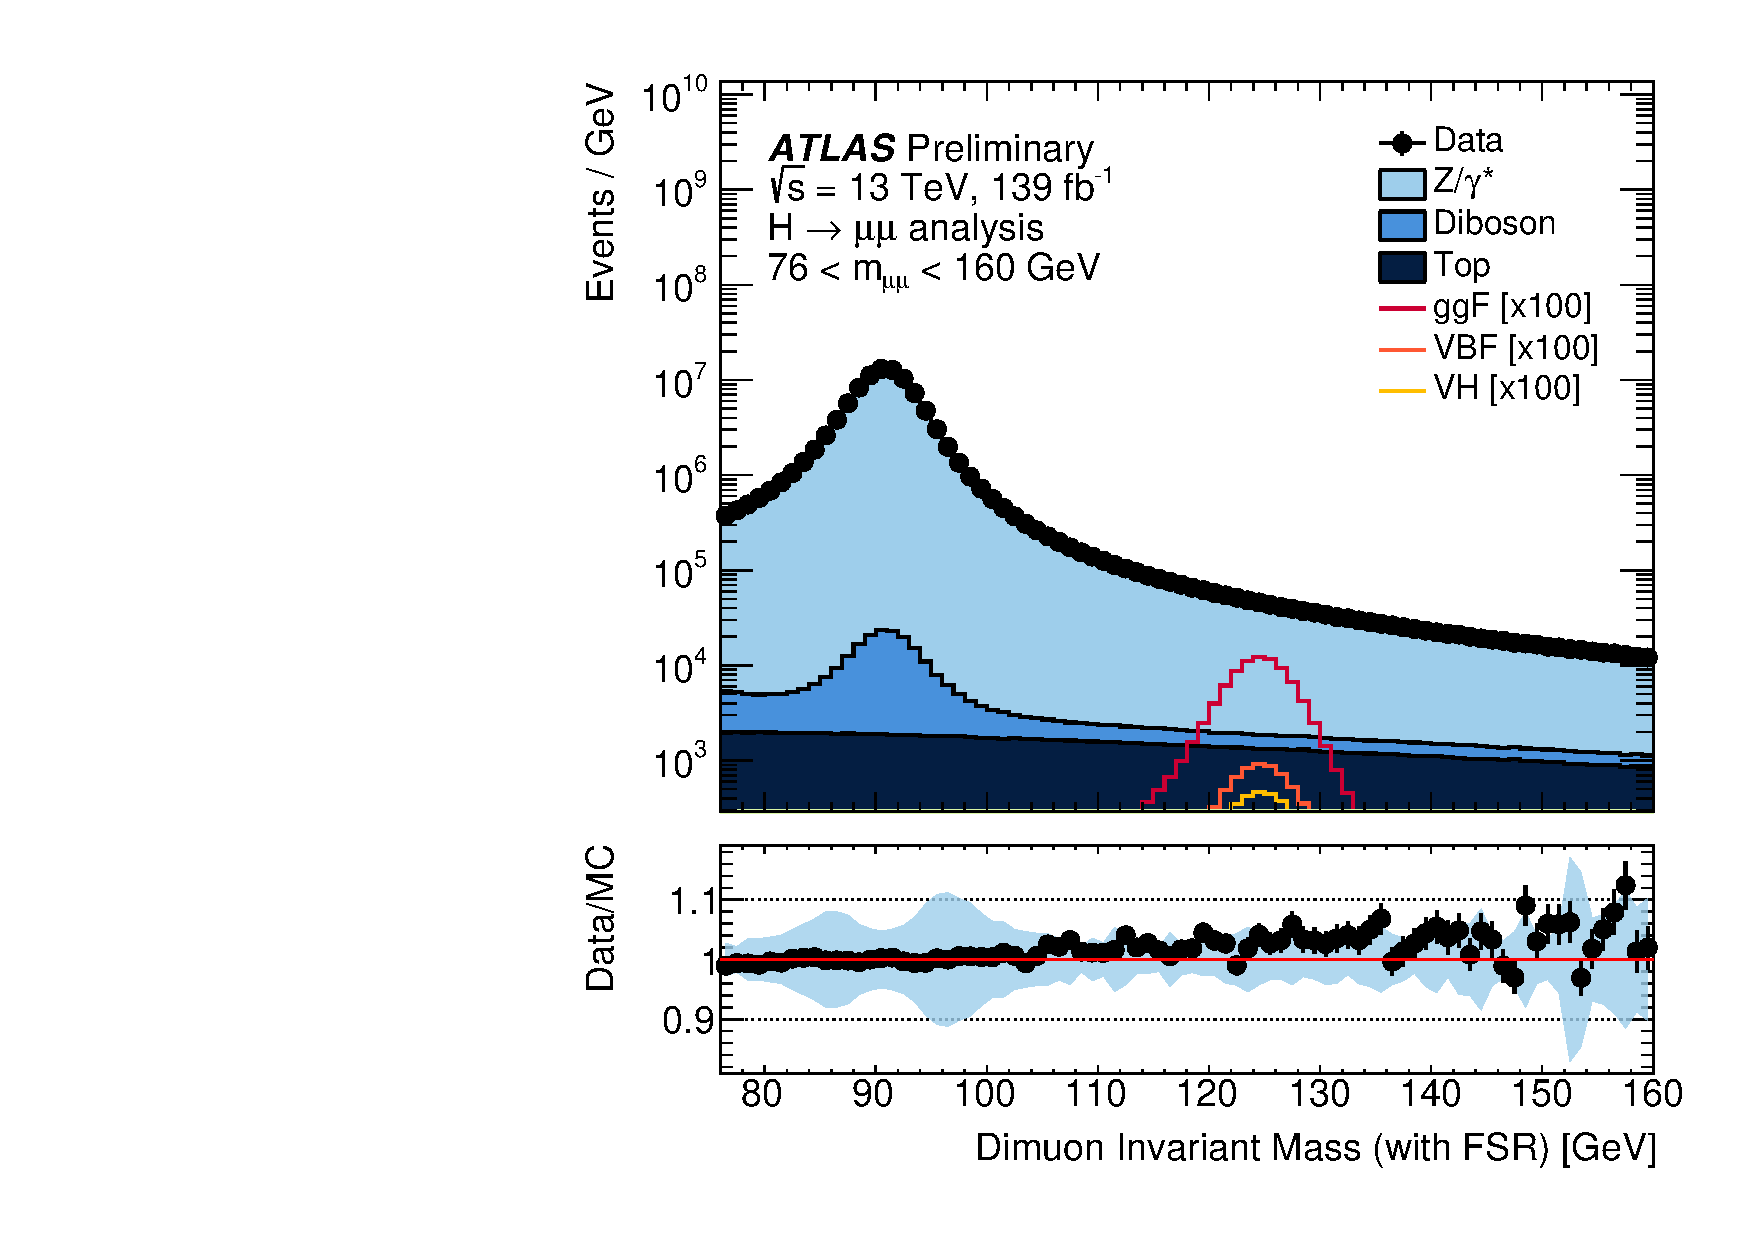
\includegraphics[width=1.0\textwidth]{figures/hmumu/sel-mmumu}
  \caption[Dimuon invariant mass spectrum of selected events.]{
  The invariant mass spectrum after the correction for
  final state radiation, for data corresponding to 139 $\ifb$.
  MC simulation is normalised to the data for easier comparison.
  Data is shown as black
  markers, the MC simulation of backgrounds, is shown as a stacked
  filled histogram, and is dominated by the DY events (light blue),
  followed by diboson (blue) and top (dark blue) contributions.
  Signal events coming from the $\ggf$, VBF, and VH production
  modes are shown as solid red, orange, and yellow lines,
  respectively, with the yields normalised to one hundred times the
  SM prediction for visibility. There are too few $\tth$ events to appear
  on the figure. The bottom panel shows the ratio between the data
  and MC simulation of background events, while the blue band
  represents the experimental systematic uncertainty. Statistical
  uncertainty on both data and MC simulation is combined in the
  error bars on data. From Ref. \cite{ATLAS-CONF-2019-028}}
  \label{fig:hmumu:sel-mmumu}
\end{figure}

\section{Event categorisation}

Data/MC:
- invariant mass spectrum
- resolution in each of the categories
- BDT output

\section{Signal modelling}

\section{Background modelling}

\section{Systematic uncertainties}

\section{Results}


